% Slides for 2025-07-22
% To create a slide, use the following:
% \begin{frame}{TITLE}
%     BODY
% \end{frame}

% To create a slide with a bullet list, use the following:
% \begin{frame}{TITLE}
%     \begin{itemize}
%         \item ITEM 1
%         \item ITEM 2
%     \end{itemize}    
% \end{frame}

% To create a slide with numbered list, use the following:
% \begin{frame}{TITLE}
%     \begin{enumerate}
%         \item ITEM 1
%         \item ITEM 2
%     \end{enumerate}
% \end{frame}

% To create a slide with a graphic:
% 1. Add the graphic to this folder (named picture.png)
% 2. Use the following:
% \begin{frame}{TITLE}
%     \centering
%     \includegraphics[height=0.7\textheight,width=0.7\textwidth,keepaspectratio]{picture.png}
% \end{frame}

% To create a slide with two columns, use the following:
% \begin{frame}{TITLE}
%     \begin{columns}
%         \begin{column}{0.5\textwidth}
%             COLUMN 1 BODY
%         \end{column}
%         \begin{column}{0.5\textwidth}
%             COLUMN 2 BODY
%         \end{column}
%     \end{columns}
% \end{frame}

\begin{frame}{ML Team Agenda}
    \begin{itemize}
        \item EGCI work
        \item Spectrogram visualization
        \item Grad-CAM
        \item Williams et al., 2025
        \item Whale detection
        \item Template matching
        \item Next steps
    \end{itemize}
\end{frame}

\begin{frame}{EGCI Work}
    \begin{figure}
        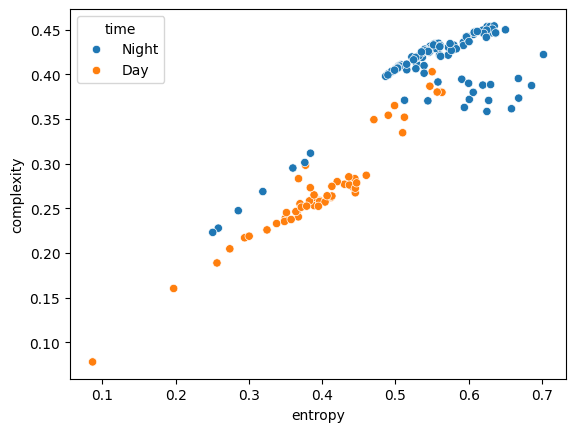
\includegraphics[height=0.7\textheight,width=0.7\textwidth,keepaspectratio]{images/muha_egci.png}
        \caption{Plot of EGCI against entropy for Muha's data, labeled with time of day}
    \end{figure}
\end{frame}

\begin{frame}{Spectrogram Visualization}
    High-dimensional spatial representation of audio clips
    \begin{figure}
        \centering
        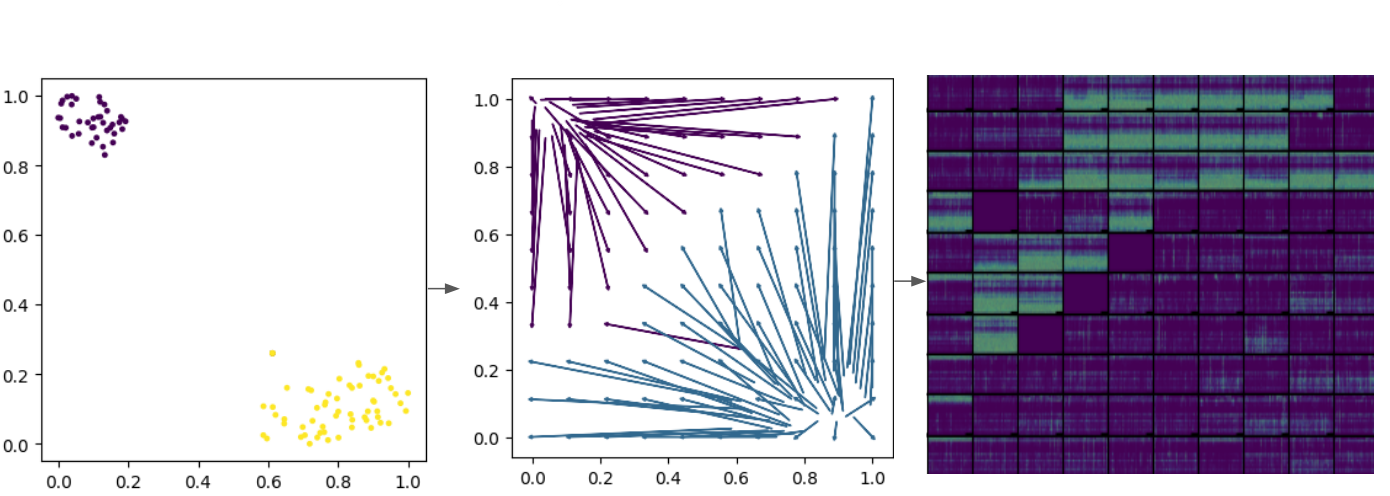
\includegraphics[height=0.85\textheight,width=0.85\textwidth,keepaspectratio]{images/spectrogram_visualization.png}
        \caption{Spectrogram visualization process of audio clips}
    \end{figure}
\end{frame}

\begin{frame}{Grad-CAM}
    \begin{columns}
        \begin{column}{0.5\textwidth}
            Degraded Grad-CAM:
            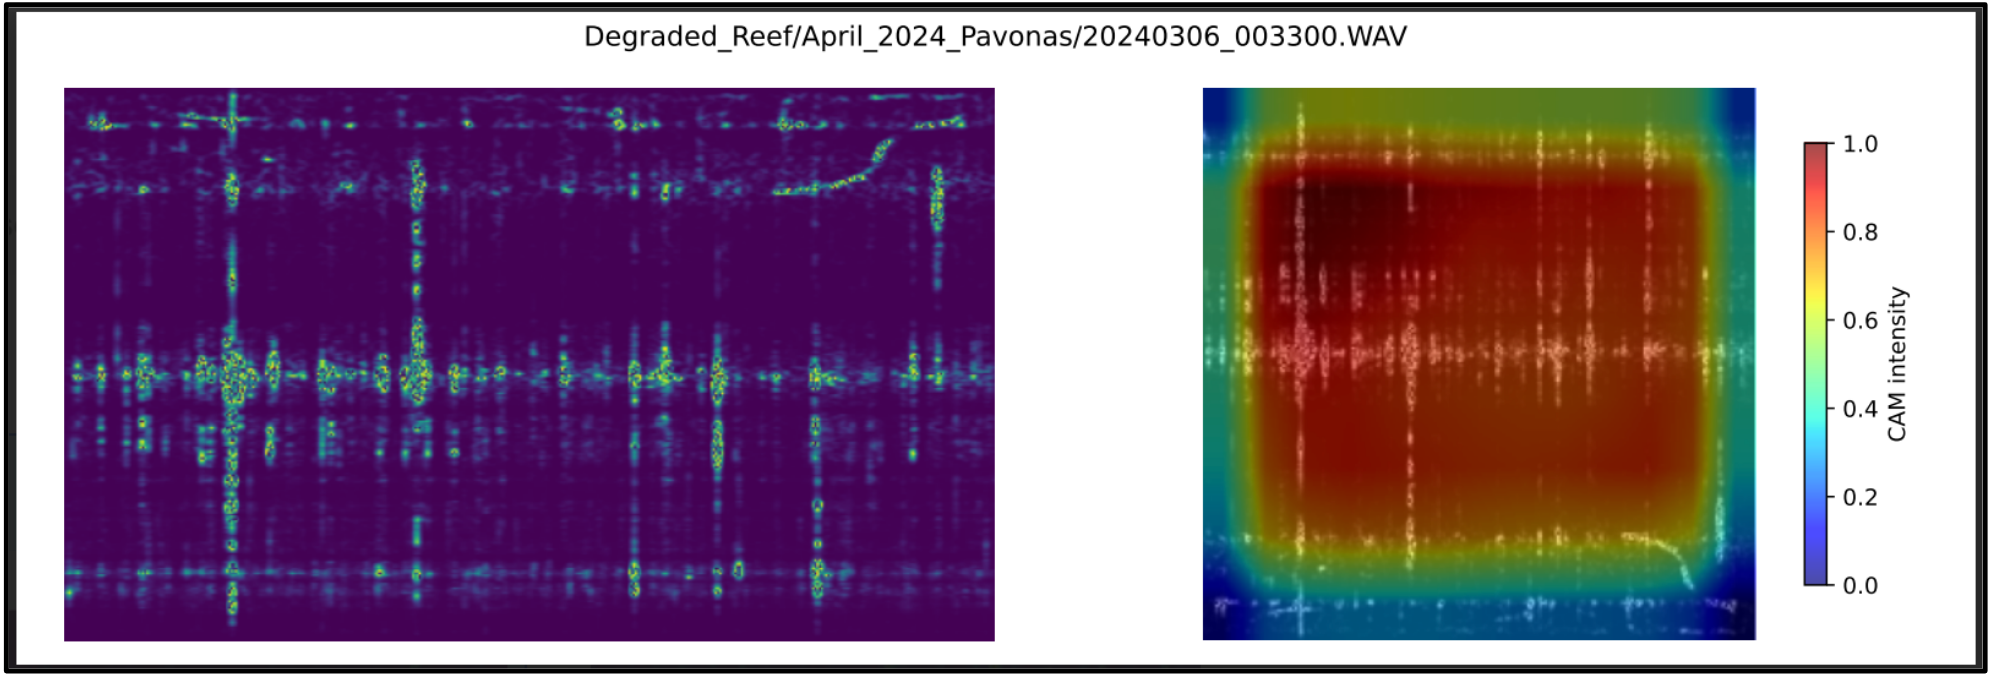
\includegraphics[height=1.0\textheight,width=1.0\textwidth,keepaspectratio]{images/degraded_grad_cam.png}
        \end{column}
        \begin{column}{0.5\textwidth}
            Non-degraded Grad-CAM:
            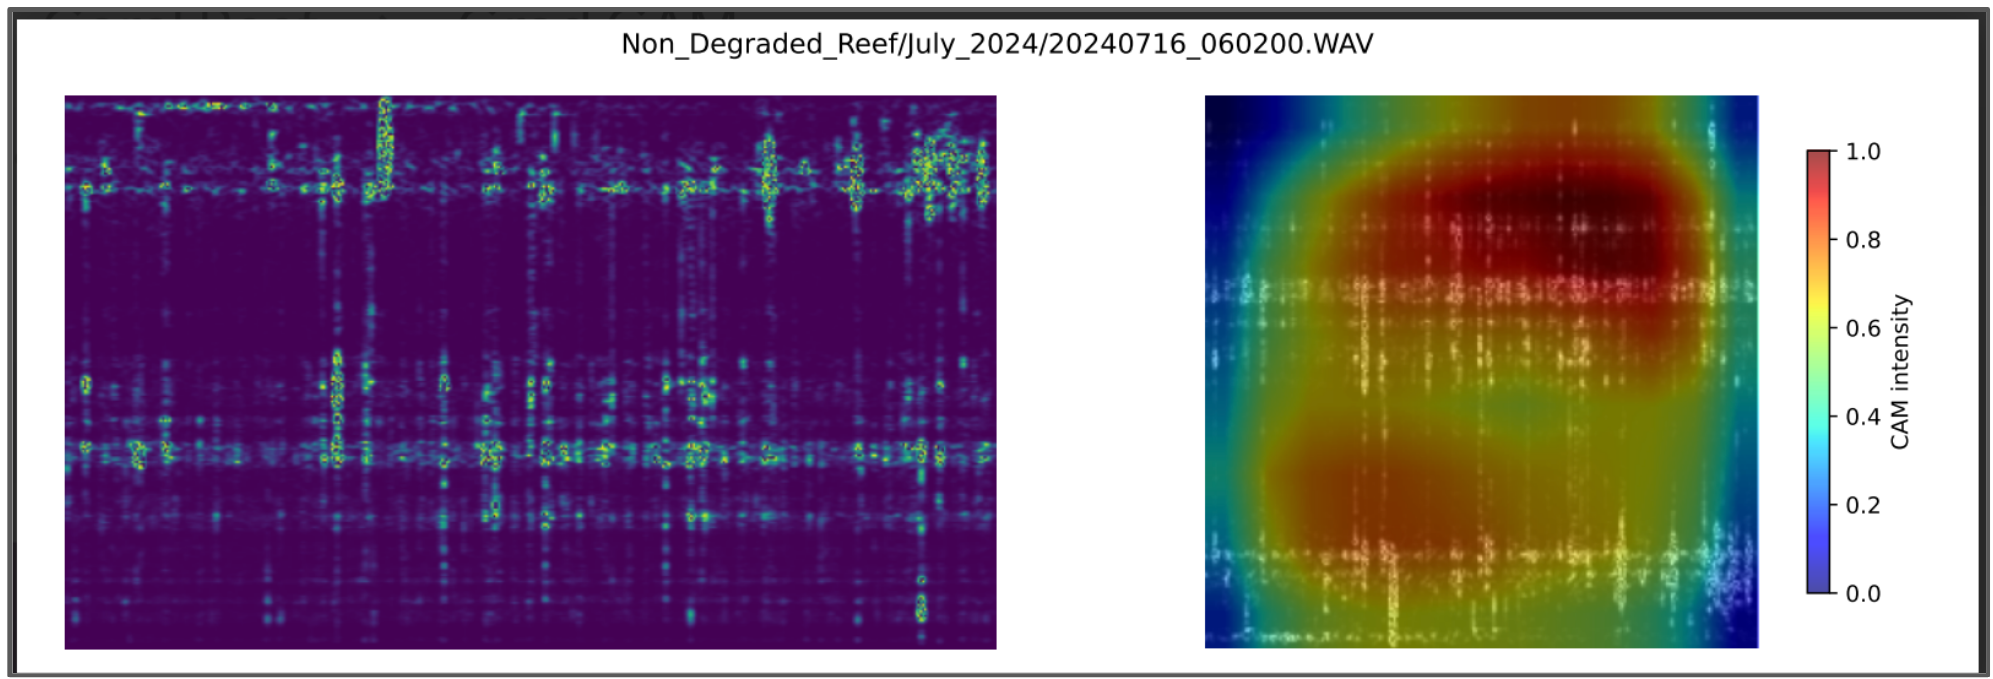
\includegraphics[height=1.0\textheight,width=1.0\textwidth,keepaspectratio]{images/non_degraded_grad_cam.png}
        \end{column}
    \end{columns}
\end{frame}

\begin{frame}{Grad-CAM Results}
    Sample of 200 degraded and non-degraded audio clips
    \begin{figure}
        \centering
        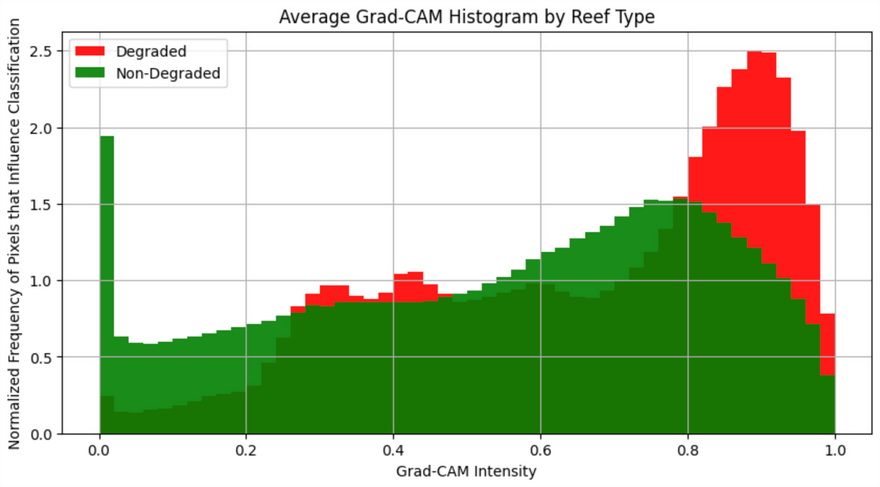
\includegraphics[height=0.6\textheight,width=0.6\textwidth,keepaspectratio]{images/grad_cam_histogram.png}
        \caption{Grad-CAM histogram}
    \end{figure}
\end{frame}

\begin{frame}{Williams et al., 2025}
    \begin{itemize}
        \item SurfPerch trained on worldwide reef sounds, tackles domain shift
        \item Using SurfPerch on Paola's data for knowledge discovery
    \end{itemize}
    \begin{columns}
        \begin{column}{0.5\textwidth}
            \begin{figure}
                \centering
                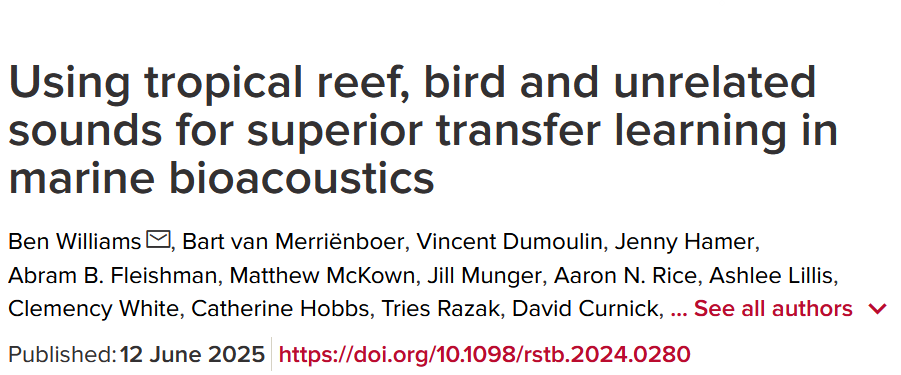
\includegraphics[height=0.8\textheight,width=0.8\textwidth,keepaspectratio]{images/Williams_et_al_2025.png}
            \end{figure}
        \end{column}
        \begin{column}{0.5\textwidth}
            \begin{figure}
                \centering
                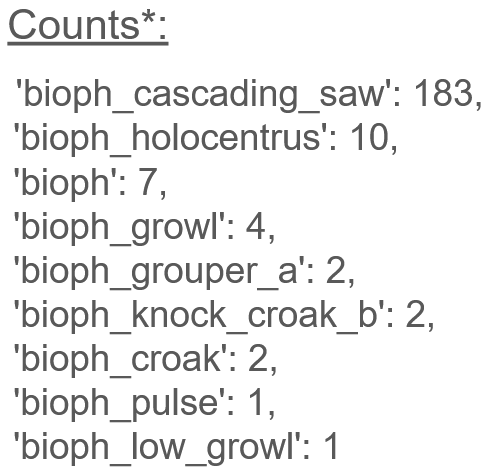
\includegraphics[height=0.5\textheight,width=0.5\textwidth,keepaspectratio]{images/surf_perch_results.png}
            \end{figure}
        \end{column}
    \end{columns}
    % Williams et al. 2025: https://royalsocietypublishing.org/doi/10.1098/rstb.2024.0280
    % SurfPerch: https://www.kaggle.com/models/google/surfperch
\end{frame}

\begin{frame}{Whale Detection}
    \begin{itemize}
        \item Can use multispecies-whale model to detect humpback whale vocalizations
        \item Issues quantifying accuracy, lack of ground truth
        \item 5\% of audio clips contain whale noises
    \end{itemize}
    \begin{figure}
        \centering
        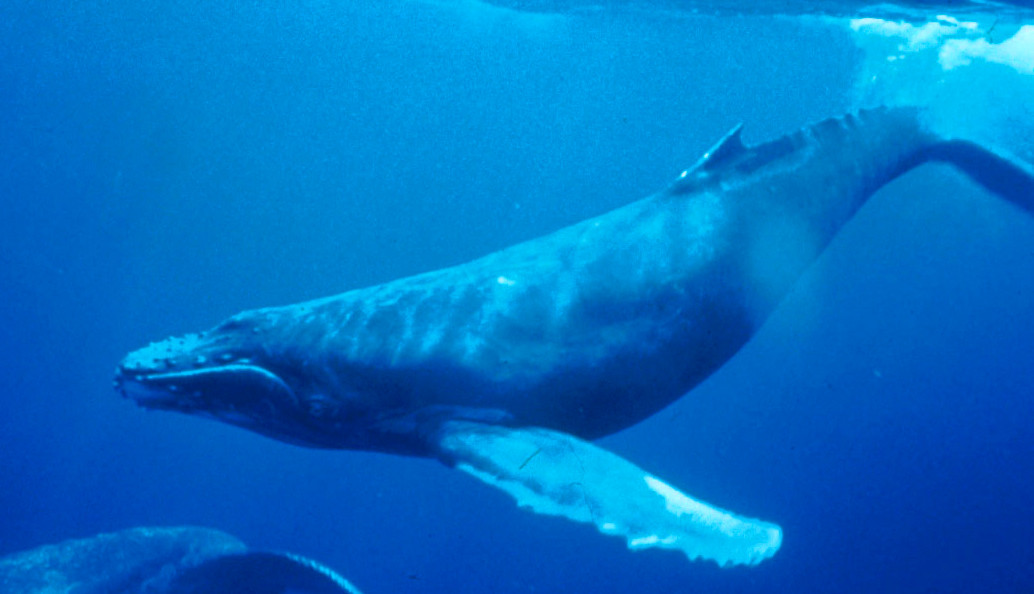
\includegraphics[height=0.4\textheight,width=0.4\textwidth,keepaspectratio]{images/humpback_whale.jpg}
        \caption{Humpback whale}
    \end{figure}
    % multispecies-whale model: https://www.kaggle.com/models/google/multispecies-whale
\end{frame}

\begin{frame}{Template Matching}
    \begin{itemize}
        \item Can take a reference sound and compare it with the data to find recordings containing said sound
        \item Implementing this with Muha's liked sounds
    \end{itemize}
\end{frame}

\begin{frame}{Next Steps}
    \begin{itemize}
        \item Create interactive website for Muha with D3.js
        \item Further work on knowledge graphs (GNNs)
        \item Continue with template matching work
    \end{itemize}
\end{frame}

\begin{frame}{Collar Team Agenda}
    \begin{itemize}
        \item Power Studies
        \begin{itemize}
            \item Power Study Overview
            \item Test Setup 
            \item In-rush Current Measurements
            \item Run Mode Configuration Measurements
        \end{itemize}
        \item Data Loss
        \begin{itemize}
            \item What is bit rot?
            \item How can we quantify and minimize data loss?
        \end{itemize}
        \item Future Plans
    \end{itemize}
\end{frame}

\begin{frame}{Power Study Overview}
    \begin{itemize}
        \item Understand power behaviour of STM32H747I-DISCO chip
        \item Measure various runtime domains for collar design metrics
        \item Combine measurements for a total power consumption estimation
    \end{itemize}
\end{frame}

\begin{frame}{Test Setup}
    \begin{itemize}
        \item Measurements taken using current clamp and pico oscilloscope
        \item Power configurations tested: Run, Sleep, Standby, Dstandby
        \item Drift issue encountered → added 10 Ohms shunt resistor in parallel with IDD
        \item Current calculated using V\_high - V\_low / 10 Ohms
    \end{itemize}  
    \includegraphics[height=0.35\textheight,width=0.7\textwidth,keepaspectratio]{images/clamp_setup.png}
    \includegraphics[height=0.35\textheight,width=0.7\textwidth,keepaspectratio]{images/shunt_setup.png}
    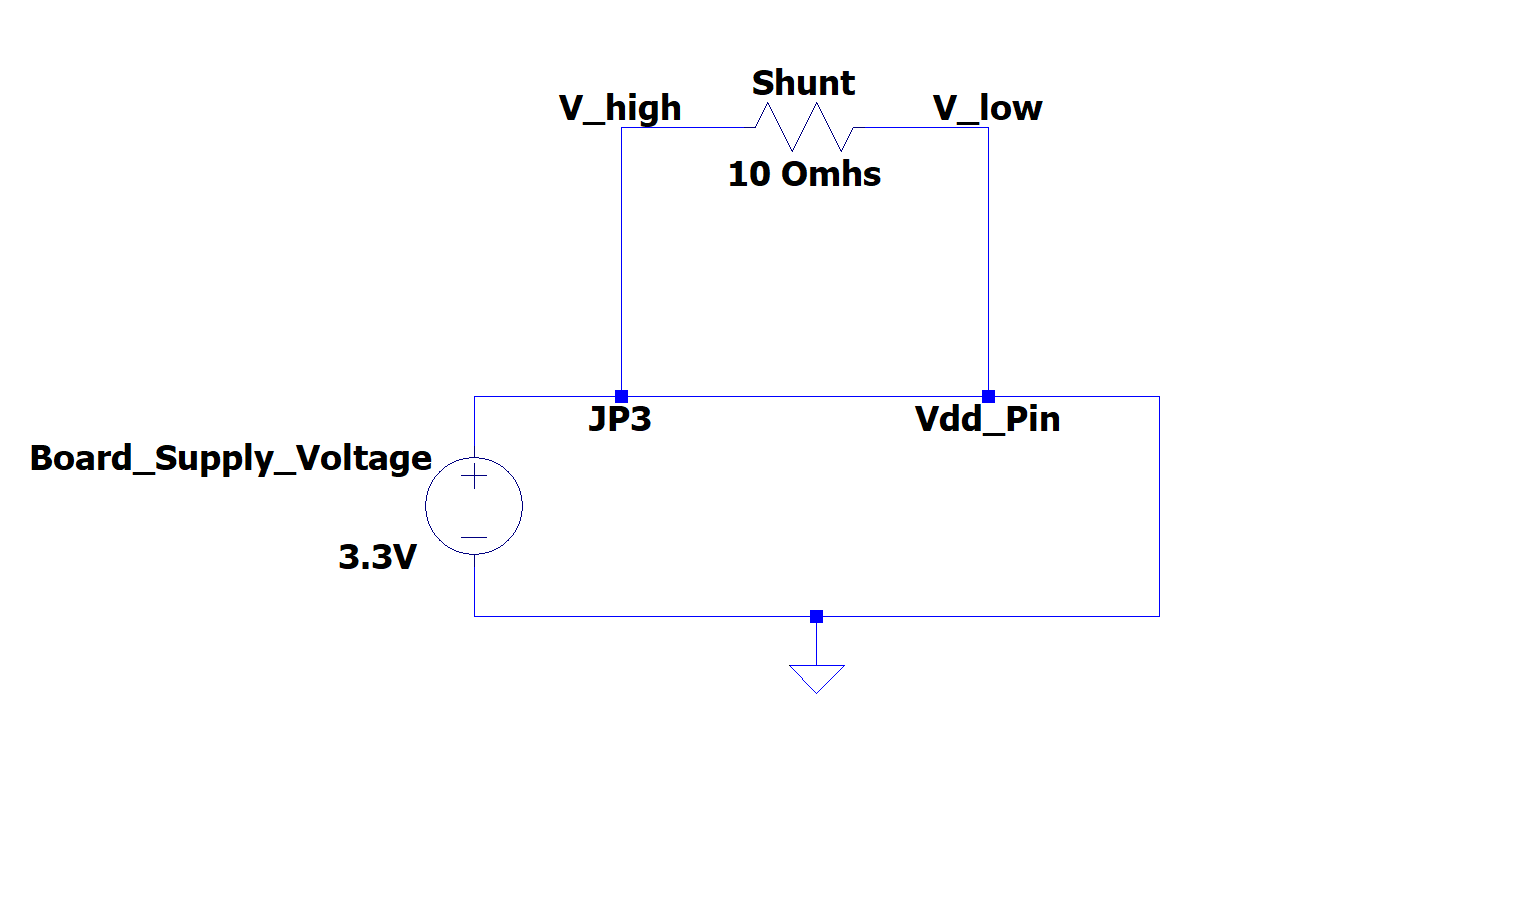
\includegraphics[height=0.35\textheight,width=0.7\textwidth,keepaspectratio]{images/shunt.png}
\end{frame}

\begin{frame}{In-Rush Current Measurements}
\begin{columns}

    % Left column: image
    \begin{column}{0.6\textwidth}
        \centering
        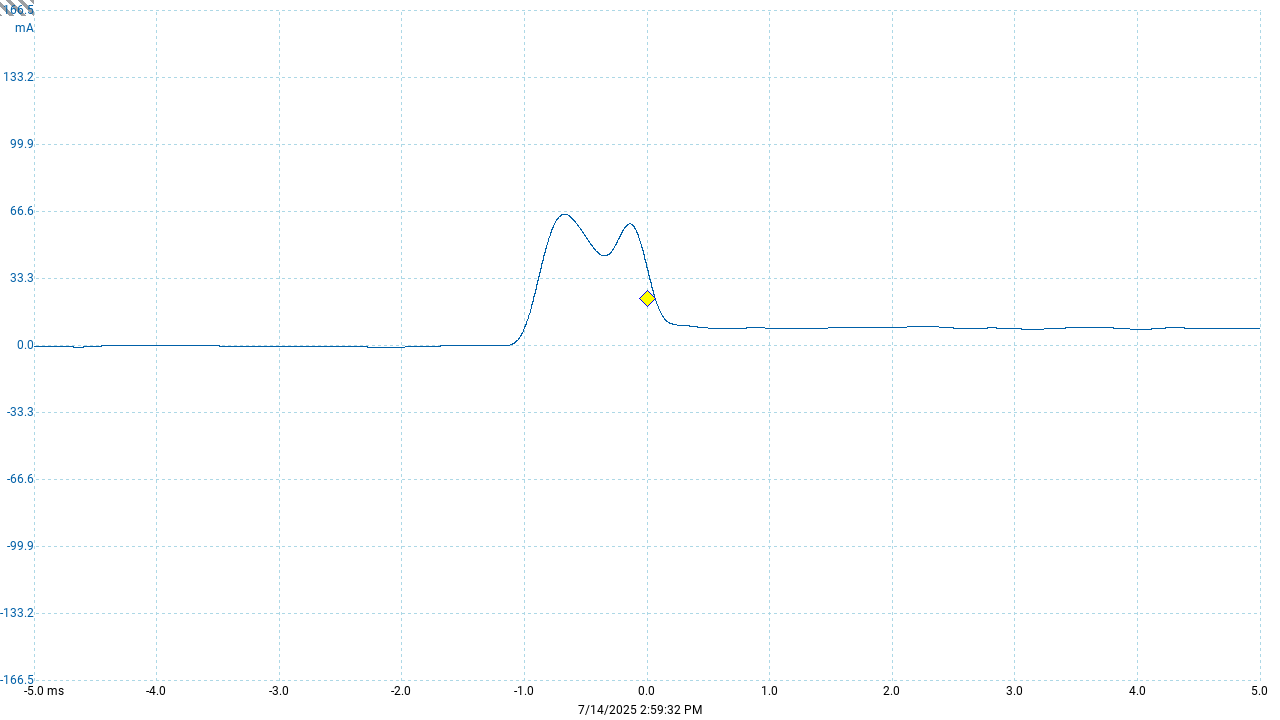
\includegraphics[width=\linewidth]{images/inrush_1core_baseline.png}
        \vspace{0.5em}
        {\small \textit{In-rush current spike at startup}}
    \end{column}

    % Right column: table
    \begin{column}{0.45\textwidth}
        \centering
        \begin{tabular}{|l|c|}
            \hline
            \textbf{Metric} & \textbf{Value} \\
            \hline
            Avg In-rush Peak 1 & 63.53 mA \\
            Avg In-rush Trough & 42.46 mA \\
            Avg In-rush Peak 2 & 58.27 mA \\
            Avg Duration     & 1.20 ms \\
            Method           & Current Clamp \\
            Trials           & 5 \\
            \hline
        \end{tabular}
        \vspace{0.5em}
        {\small \textit{In-rush Average Metrics}}
    \end{column}
\end{columns}
\end{frame}

\begin{frame}{Run Mode Configuration Measurements}
    \begin{itemize}
        \item 
    \end{itemize}
    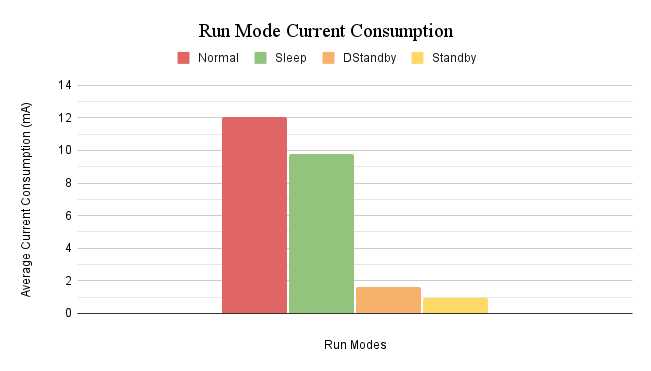
\includegraphics[height=0.5\textheight,width=0.9\textwidth,keepaspectratio]{images/run_modes.png}
\end{frame}

\begin{frame}{What is Bit Rot?}
    \begin{itemize}
        \item Digital data slowly corrupting overtime
        \item It occurs when: hold
    \end{itemize}
    \centering
    % \includegraphics[height=0.7\textheight,width=0.7\textwidth,keepaspectratio]{picture.png}
\end{frame}

\begin{frame}{Types of NAND Flash}
    \centering
    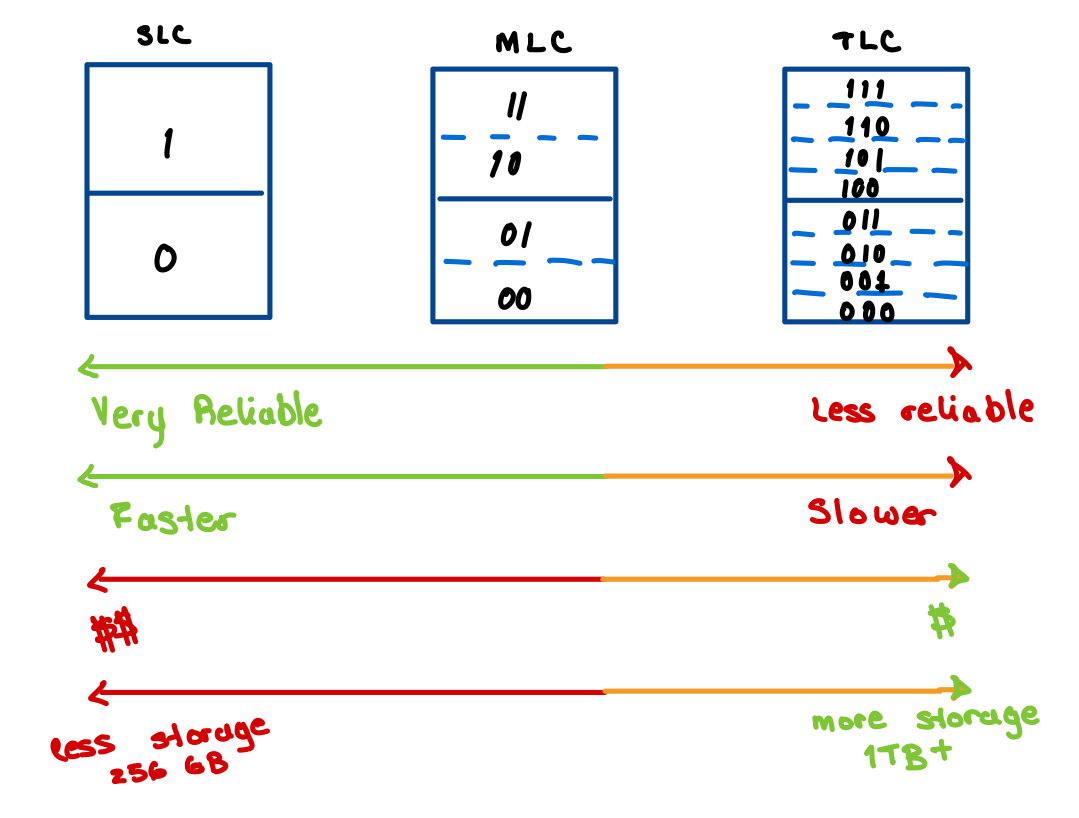
\includegraphics[height=0.9\textheight,width=0.9\textwidth,keepaspectratio]{images/flash_types.png}
\end{frame}

\begin{frame}{Maintaining Data Integrity}
    Managing data loss on three levels:
    \begin{itemize}
        \item \textbf{Hardware:} Use of ECC (Error-Correcting Code)
        \item \textbf{File System:} Use of error checking file systems eg. ZFS, ext4
        \item \textbf{File/Page:} Use of checksums and hashes
    \end{itemize}
    % \includegraphics[height=0.7\textheight,width=0.7\textwidth,keepaspectratio]{picture.png}
\end{frame}

\begin{frame}{Fermi Estimations}
    \begin{itemize}
        \item \textbf{SD card size:} will likely need something of the three digit magnitude or more
        \item \textbf{Battery:} 3-4 lbs
        \item Overhead to consider: compressing files to .flac, power fail safe
    \end{itemize}
\end{frame}

\begin{frame}{What's next?}
    \begin{itemize}
        \item Keep researching ways to minimize data loss
        \item Get clarification from collaborators on what amount of data loss is acceptable and what type of data they want to collect
        \item Write a script to visualize data loss rate
    \end{itemize}
\end{frame}
